%%%%%%%%%%%%%%%%%%%%%%%%%%%%%%%%%%%%%%%%%
% Short Sectioned Assignment LaTeX Template Version 1.0 (5/5/12)
% This template has been downloaded from: http://www.LaTeXTemplates.com
% Original author:  Frits Wenneker (http://www.howtotex.com)
% License: CC BY-NC-SA 3.0 (http://creativecommons.org/licenses/by-nc-sa/3.0/)
%%%%%%%%%%%%%%%%%%%%%%%%%%%%%%%%%%%%%%%%%

%----------------------------------------------------------------------------------------
%	PACKAGES AND OTHER DOCUMENT CONFIGURATIONS
%----------------------------------------------------------------------------------------

\documentclass[paper=a4, fontsize=11pt]{scrartcl} % A4 paper and 11pt font size

% ---- Entrada y salida de texto -----

\usepackage[T1]{fontenc} % Use 8-bit encoding that has 256 glyphs
\usepackage[utf8]{inputenc}
%\usepackage{fourier} % Use the Adobe Utopia font for the document - comment this line to return to the LaTeX default

% ---- Idioma --------

\usepackage[spanish, es-tabla]{babel} % Selecciona el español para palabras introducidas automáticamente, p.ej. "septiembre" en la fecha y especifica que se use la palabra Tabla en vez de Cuadro

% ---- Otros paquetes ----

\usepackage{url} % ,href} %para incluir URLs e hipervínculos dentro del texto (aunque hay que instalar href)
\usepackage{amsmath,amsfonts,amsthm} % Math packages
%\usepackage{graphics,graphicx, floatrow} %para incluir imágenes y notas en las imágenes
\usepackage{graphics,graphicx, float} %para incluir imágenes y colocarlas

% Para hacer tablas comlejas
%\usepackage{multirow}
%\usepackage{threeparttable}

%\usepackage{sectsty} % Allows customizing section commands
%\allsectionsfont{\centering \normalfont\scshape} % Make all sections centered, the default font and small caps

\usepackage{fancyhdr} % Custom headers and footers
\pagestyle{fancyplain} % Makes all pages in the document conform to the custom headers and footers
\fancyhead{} % No page header - if you want one, create it in the same way as the footers below
\fancyfoot[L]{} % Empty left footer
\fancyfoot[C]{} % Empty center footer
\fancyfoot[R]{\thepage} % Page numbering for right footer
\renewcommand{\headrulewidth}{0pt} % Remove header underlines
\renewcommand{\footrulewidth}{0pt} % Remove footer underlines
\setlength{\headheight}{13.6pt} % Customize the height of the header

\numberwithin{equation}{section} % Number equations within sections (i.e. 1.1, 1.2, 2.1, 2.2 instead of 1, 2, 3, 4)
\numberwithin{figure}{section} % Number figures within sections (i.e. 1.1, 1.2, 2.1, 2.2 instead of 1, 2, 3, 4)
\numberwithin{table}{section} % Number tables within sections (i.e. 1.1, 1.2, 2.1, 2.2 instead of 1, 2, 3, 4)

\setlength\parindent{0pt} % Removes all indentation from paragraphs - comment this line for an assignment with lots of text

\newcommand{\horrule}[1]{\rule{\linewidth}{#1}} % Create horizontal rule command with 1 argument of height

\graphicspath{ {./images/} }
\usepackage{subcaption}
\usepackage{hyperref}
\usepackage{soul}


%----------------------------------------------------------------------------------------
%	TÍTULO Y DATOS DEL ALUMNO
%----------------------------------------------------------------------------------------

\title{	
\normalfont \normalsize 
\textsc{\textbf{Aprendizaje Automático (2019)} \\ Doble Grado en Ingeniería Informática y Matemáticas \\ Universidad de Granada} \\ [25pt] % Your university, school and/or department name(s)
\horrule{0.5pt} \\[0.4cm] % Thin top horizontal rule
\huge Memoria Práctica 3 \\ % The assignment title
\horrule{2pt} \\[0.5cm] % Thick bottom horizontal rule
}

\author{Luis Balderas Ruiz \\ \texttt{luisbalderas@correo.ugr.es}} 
 % Nombre y apellidos 


\date{\normalsize\today} % Incluye la fecha actual

%----------------------------------------------------------------------------------------
% DOCUMENTO
%----------------------------------------------------------------------------------------

\begin{document}

\maketitle % Muestra el Título

\newpage %inserta un salto de página

\tableofcontents % para generar el índice de contenidos

\listoffigures

\listoftables

\newpage


%----------------------------------------------------------------------------------------
%	Introducción
%----------------------------------------------------------------------------------------

\section{Recognition of handwritten digits}

\subsection{Introducción}

Nos enfrentamos a un problema de clasificación multietiqueta (9 clases) sobre una base de datos de reconocimiento de dígitos manuscritos, proveniente de la Universidad de Bogazici. Tras extraer mapas de bits de dimensión $32\times32$ normalizados, se dividen en bloques de $4\times4$ disjuntos y se cuenta el número de píxeles en cada bloque. Esto genera una matriz $8\times8$ con entrada en los números enteros del 0 al 16. Más información en \cite{optdigits.names}. 

\subsection{Preprocesado}

El preprocesado de los datos es la parte más importante del pipeline en un proyecto de ciencia de datos. De él se espera refinar, ajustar, completar y, en definitiva, mejorar la congruencia y consistencia de los mismos para conseguir mejores resultados en la parte de análisis y clasificación. Para conseguir un preprocesado más acertado, me baso continuamente en distintas visualizaciones que arrojen pistas sobre los pasos a seguir. Propongo los siguientes apartados:

\subsubsection{Balanceo de las clases} 

Un dataset balanceado es primordial para garantizar un correcto aprendizaje del modelo. En caso de desbalanceo, las clases más representadas tendrían un peso mayor a la hora de etiquetar instancias nuevas en test, de forma que las menos representadas acabarían, con gran probabilidad, mal clasificadas. Cuando se da desbalanceo hay dos posibles alternativas: eliminar instancias de las clases más repetidas (undersampling) o generar nuevas de las clases minoritarias (oversampling). En este último caso, se suelen utilizar algoritmos como SMOTE (\cite{smote}). \\

En nuestro caso, las clases están absolutamente balanceadas:

\begin{table}[H]
	\centering
	\begin{tabular}{|c|c|}
		\hline
		Etiqueta & Número de instancias \\ \hline
		0        & 178                  \\ \hline
		1        & 182                  \\ \hline
		2        & 177                  \\ \hline
		3        & 183                  \\ \hline
		4        & 181                  \\ \hline
		5        & 182                  \\ \hline
		6        & 181                  \\ \hline
		7        & 179                  \\ \hline
		8        & 174                  \\ \hline
		9        & 180                  \\ \hline
	\end{tabular}
\end{table}

Veámoslo también gráficamente:

\begin{figure}[H] %con el [H] le obligamos a situar aquí la figura
	\centering
	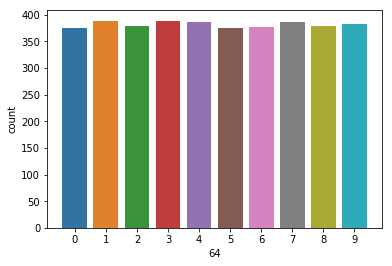
\includegraphics[scale=0.6]{count-clases.png}  %el parámetro scale permite agrandar o achicar la imagen. En el nombre de archivo puede especificar directorios
	\caption{Histograma con el número de instancias por clase} 
	\label{fig:clases}
\end{figure}

Por tanto, no es necesario hacer ninguna modificación en ese sentido.

\subsubsection{Selección de características: Variabilidad de los datos}

A continuación, estudiamos la calidad de las características (columnas en la matriz). Para ello, realizo una descripción estadística de los datos. De las 63 características se estudia la variabilidad de cada individuo a través de la media, la desviación típica, el recorrido intercuartílico, máximo, mínimo... Represento la matriz de correlación para estudiar la correlación lineal entre las características:

\begin{figure}[H] %con el [H] le obligamos a situar aquí la figura
	\centering
	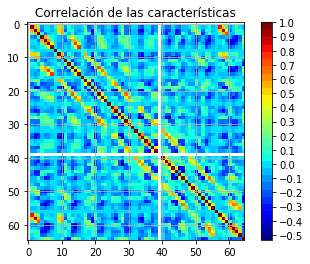
\includegraphics[scale=0.8]{corr-matrix.png}  %el parámetro scale permite agrandar o achicar la imagen. En el nombre de archivo puede especificar directorios
	\caption{Matriz de correlación de características} 
	\label{fig:corr-mat}
\end{figure}


\section{Airfoil self noise}
\newpage
\section{Bibliografía}

%------------------------------------------------

\bibliography{citas} %archivo citas.bib que contiene las entradas 
\bibliographystyle{plain} % hay varias formas de citar

\end{document}
